% 	Name		:: 	sthlm Beamer Theme  HEAVILY based on the hsrmbeamer theme (Benjamin Weiss)
%	Author		:: 	Mark Hendry Olson (mark@hendryolson.com)
%	Created		::	2013-07-31
%	Updated		::	June 18, 2015 at 08:45
%	Version		:: 	1.0.2
%	Email		:: 	hendryolson@gmail.com
%	Website		:: 	http://v42.com
%
% 	License		:: 	This file may be distributed and/or modified under the
%                  	GNU Public License.
%
%	Description	::	This presentation is a demonstration of the sthlm beamer
%					theme, which is HEAVILY based on the HSRM beamer theme created by Benjamin Weiss
%					(benjamin.weiss@student.hs-rm.de), which can be found on GitHub
%					<https://github.com/hsrmbeamertheme/hsrmbeamertheme>.


%-=-=-=-=-=-=-=-=-=-=-=-=-=-=-=-=-=-=-=-=-=-=-=-=
%
%        LOADING DOCUMENT
%
%-=-=-=-=-=-=-=-=-=-=-=-=-=-=-=-=-=-=-=-=-=-=-=-=

\documentclass[newPxFont]{beamer}
\usetheme{sthlm}
%\usecolortheme{sthlmv42}

%-=-=-=-=-=-=-=-=-=-=-=-=-=-=-=-=-=-=-=-=-=-=-=-=
%        LOADING PACKAGES
%-=-=-=-=-=-=-=-=-=-=-=-=-=-=-=-=-=-=-=-=-=-=-=-=
\usepackage[utf8]{inputenc}
\usepackage[T1]{fontenc}

%\usepackage{chronology}
\usepackage{chronosys}
\usepackage{subfigure}

\newcommand{\tabitem}{%
  \usebeamertemplate{itemize item}\hspace*{\labelsep}}


%\renewcommand{\event}[3][e]{%
%  \pgfmathsetlength\xstop{(#2-\theyearstart)*\unit}%
%  \ifx #1e%
%    \draw[fill=black,draw=none,opacity=0.5]%
%      (\xstop, 0) circle (.2\unit)%
%      node[opacity=1,rotate=45,right=.2\unit] {#3};%
%  \else%
%    \pgfmathsetlength\xstart{(#1-\theyearstart)*\unit}%
%    \draw[fill=black,draw=none,opacity=0.5,rounded corners=.1\unit]%
%      (\xstart,-.1\unit) rectangle%
%      node[opacity=1,rotate=45,right=.2\unit] {#3} (\xstop,.1\unit);%
%  \fi}%

%-=-=-=-=-=-=-=-=-=-=-=-=-=-=-=-=-=-=-=-=-=-=-=-=
%        BEAMER OPTIONS
%-=-=-=-=-=-=-=-=-=-=-=-=-=-=-=-=-=-=-=-=-=-=-=-=

%\setbeameroption{show notes}

%-=-=-=-=-=-=-=-=-=-=-=-=-=-=-=-=-=-=-=-=-=-=-=-=
%
%	PRESENTATION INFORMATION
%
%-=-=-=-=-=-=-=-=-=-=-=-=-=-=-=-=-=-=-=-=-=-=-=-=

\title{Lost in Navigation?}
\subtitle{Ensuring Living Lab Frameworks Stay on Course with Local Needs}
%\date{\small{\jobname}}
%\date{\today}
\author{\texttt{E. Delay} \texttt{A.Hertzog-Adamczewski}, \texttt{R. Duboz}, \texttt{A. Ogilvie}, \texttt{W. Daré}, \texttt{A. Bah}, \texttt{O. Samaké}}
\institute{CIRAD -- IRD -- UCAD -- SAED}

\hypersetup{
pdfauthor = {E. DELAY},
pdfsubject = {IFALL - Bordeau.},
pdfkeywords = {Living-Labs, Santés et Territoires, One-Health},
pdfmoddate= {\pdfdate},
pdfcreator = {}
}

\begin{document}

%-=-=-=-=-=-=-=-=-=-=-=-=-=-=-=-=-=-=-=-=-=-=-=-=
%
%	TITLE PAGE
%
%-=-=-=-=-=-=-=-=-=-=-=-=-=-=-=-=-=-=-=-=-=-=-=-=


\maketitle


%-=-=-=-=-=-=-=-=-=-=-=-=-=-=-=-=-=-=-=-=-=-=-=-=
%	FRAME: INTRODUCTION
%-=-=-=-=-=-=-=-=-=-=-=-=-=-=-=-=-=-=-=-=-=-=-=-=

\section{Introduction :\\ Inscription}

\begin{frame}[c]{A Project Supporting Transitions}
  \vspace{-0.5cm}
  \begin{columns}[onlytextwidth,T]
    \column{\dimexpr\linewidth-30mm-5mm}

    \textbf{Main objective:} to support \textbf{agroecological transitions} through the establishment of \textit{Living Labs}.

    \begin{itemize}
      \item Co-construction of knowledge and practices.
      \item Experimentation in real-world conditions with local stakeholders.
      \item Production of solutions adapted to specific territories.
    \end{itemize}

    \vspace{0.3cm}
    Embedded within the \textbf{One Health} framework: human, animal, environment.

    \column{30mm}
    %\vspace{0.5cm}
    % Optional illustrative image
    \includegraphics[height=7.5cm]{img/diohine.jpg}
  \end{columns}
\end{frame}

\section{Theoretical Framework \& Method}

\begin{frame}[c]{Theoretical Framework: Assemblage Approach}
  \vspace{-0.5cm}
  \begin{columns}[onlytextwidth,T]
    \column{\dimexpr\linewidth-30mm-5mm}

    The \textbf{assemblage approach} views reality as \textbf{dynamic configurations} 
    that combine heterogeneous elements:
    \begin{itemize}
      \item humans and non-humans,
      \item material and immaterial,
      \item discourses and practices.
    \end{itemize}

    \vspace{0.3cm}
    According to Hertz \& Bousquet (2025), the specificity of assemblages lies in their
    ability to generate \textbf{affect}: an experiential intensity that can 
    \textbf{trigger situated action}.
    
    \vspace{0.3cm}
    → Importance of \textit{affective knowing}: knowledge must be \textit{felt and experienced}
    in order to become transformative.

    \column{30mm}
    %\vspace{1.5cm}
    % Optional illustrative image
    \includegraphics[height=7.5cm]{img/diohine_liens}
  \end{columns}
\end{frame}

\begin{frame}[c]{Theoretical Framework: constitutional moments}
  \vspace{-0.5cm}
  \begin{columns}[onlytextwidth,T]
    \column{\dimexpr\linewidth-30mm-5mm}

    Our methodological approach:
    \begin{itemize}
      \item \textbf{Longitudinal observation} of the project in Senegal.
      \item Analysis of \textbf{grey literature}: more than 2,400 documents 
            (reports, notes, presentations, etc.).
      \item Attention to \textbf{“constitutional moments”} 
            (Jasanoff, 2011): situations where established frames break down 
            and new meanings emerge.
    \end{itemize}

    \vspace{0.3cm}
    These moments reveal how affect and local imaginaries reshape 
    arrangements and trigger transformations.

    \column{30mm}
    \vspace{1.5cm}
    % Optional illustrative image
    % \includegraphics[height=3.5cm]{img/methodology.png}
  \end{columns}
\end{frame}

\section{Case Study: Living Labs in the Senegal Context}

\begin{frame}[c]{Chronology of the Living Labs}
  \vspace{-0.5cm}
  

    \begin{itemize}
      \item \textbf{Phase 1: Diagnosis} – initial mapping of localities and actors.  
      \item \textbf{Phase 2: Progressive integration} – emergence of groups, 
            opening of arenas such as \textit{Kourel} (village forums).  
      \item \textbf{Phase 3: Rooted activities \& unexpected synergies} – 
            interactions deepened, new alignments and collaborations emerged.  
    \end{itemize}

    \vspace{0.3cm}
    → Living Labs evolved from dispersed elements to concrete 
    \textbf{assemblages in action}.

\end{frame}

\begin{frame}[c]{Initial Phase: Disjointed Elements}
  \vspace{-0.5cm}
  \begin{columns}[onlytextwidth,T]
    \column{\dimexpr\linewidth-30mm-5mm}

    \begin{itemize}
      \item \textbf{Multiplicity of visions and definitions of “participation”}.\\  
            → Ranging from consultation to co-decision or instrumental mobilization.  
      \item Divergences among thematic groups  
            (e.g. animal health, human health, aquatic biodiversity, food systems).  
      \item Common keywords circulated (“participation”, “One Health”), 
            but meanings varied and sometimes conflicted.  
    \end{itemize}

    → The phase was marked by dispersion, inertia, and misunderstandings.

    \column{30mm}
    %\vspace{1.5cm}
    % Optional table or diagram of divergences
    \includegraphics[height=8.5cm]{img/bus_mbane}
  \end{columns}
\end{frame}

\begin{frame}[c]{Intermediate Phase: First Convergences}
  \vspace{-0.5cm}
  \begin{columns}[onlytextwidth,T]
    \column{\dimexpr\linewidth-30mm-5mm}

    \begin{itemize}
      \item \textbf{Mergers of groups}: e.g. \textit{Pesticides} + \textit{Soil–Plant} 
            → formation of the \textbf{Agro-Aquaculture Farm}.  
      \item \textbf{Tensions and debates}:  
            – Productivist logics (seeds, mechanization, yields)  
            – Agroecological orientations (sustainability, circular practices).  
      \item Participatory practices created \textbf{new alliances}, 
            while some divergences persisted.  
    \end{itemize}

    \vspace{0.3cm}
    → First steps from dispersion toward collective identities and shared perspectives.

    \column{30mm}
    
    % Optional diagram of group mergers
    \includegraphics[height=7.5cm]{img/mobiliette_mbane}
  \end{columns}
\end{frame}

\begin{frame}[c]{Advanced Phase: Assemblage in Action}
  \vspace{-0.5cm}
  \begin{columns}[onlytextwidth,T]
    \column{\dimexpr\linewidth-30mm-5mm}

    \begin{itemize}
      \item \textbf{Concrete alignments}:  
            – Fodder crops,  
            – Integrated agro-aquaculture farms,  
            – Fish ponds as alternatives to declining catches.  
      \item \textbf{Synergies across groups} emerged, 
            transcending disciplinary and institutional boundaries.  
      \item Activities rooted in local contexts validated earlier 
            experimental bets and strengthened collective ownership.  
    \end{itemize}

    \vspace{0.3cm}
    → From abstract discussions to \textbf{operational assemblages in the field}.

    \column{30mm}
    % Optional illustrative diagram
    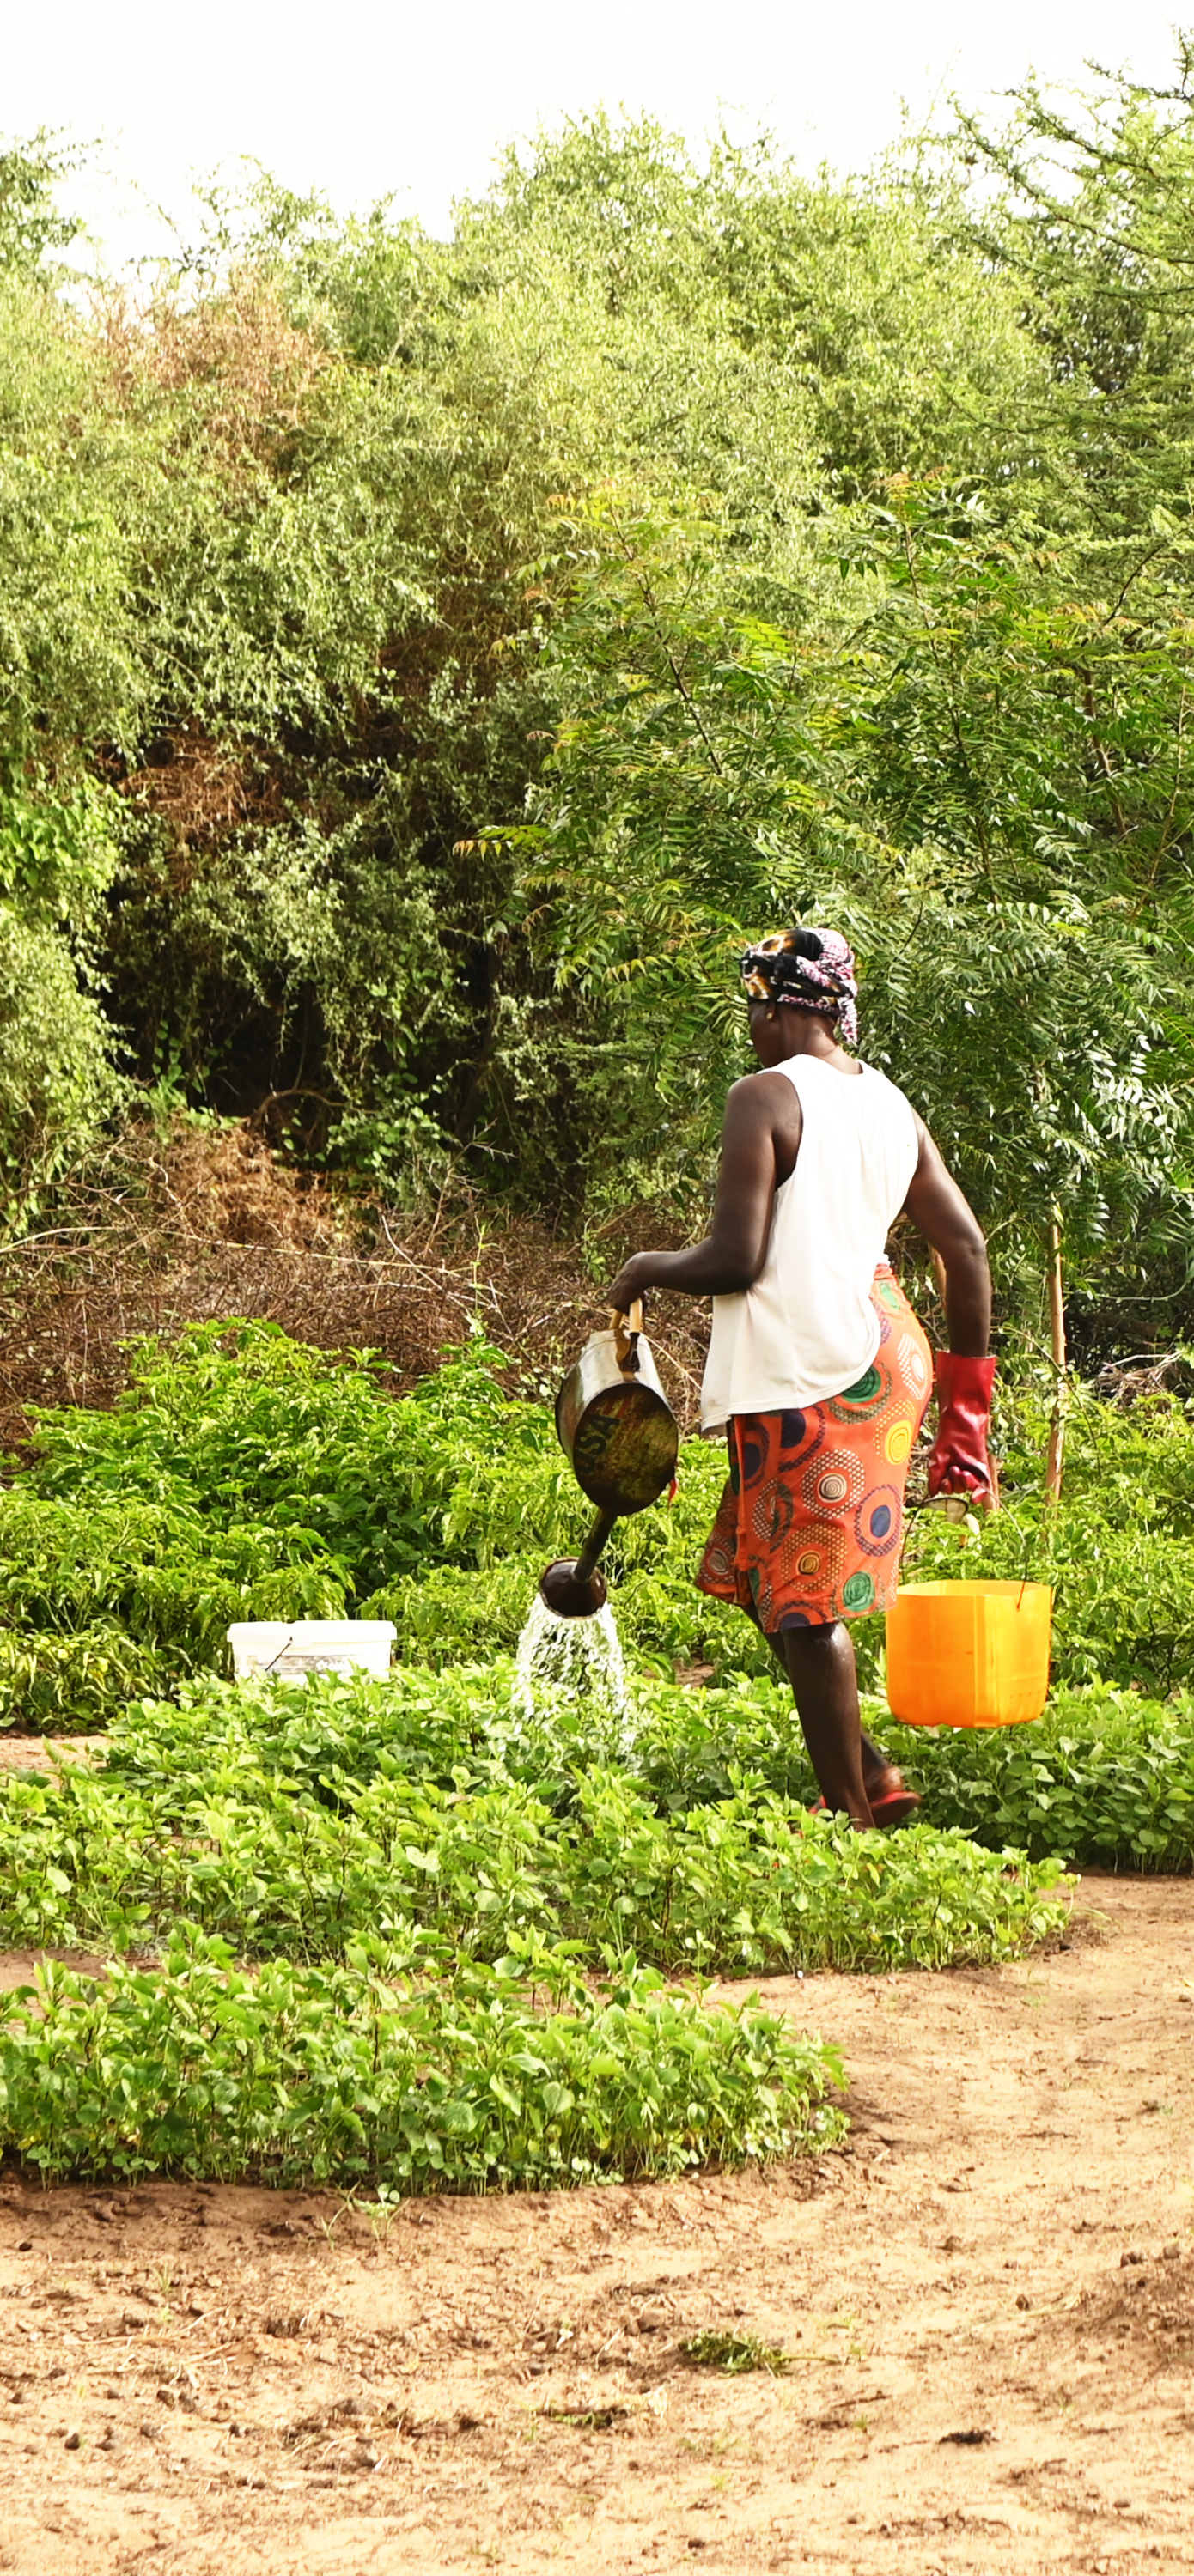
\includegraphics[height=7.5cm]{img/arrodage_mbane}
  \end{columns}
\end{frame}

\section{Findings \& Discussion}

\begin{frame}[c]{Alignements and Assemblage}
  \begin{center}
    \includegraphics[width=\textwidth]{img/Drawing 2025-09-07 11.03.30.excalidraw}
  \end{center}
  
\end{frame}

\begin{frame}[c]{Role of Affects in Reconfigurations}
  \vspace{-0.5cm}
  \begin{columns}[onlytextwidth,T]
    \column{\dimexpr\linewidth-30mm-5mm}

    \textbf{Triggering moments:}
    \begin{itemize}
      \item Revelation of \textbf{chemical pollution} in Lake Guiers.  
      \item \textbf{Conflicts} between indigenous and non-indigenous fishers.  
      \item Collective enthusiasm for \textbf{fodder crop experimentation}.  
    \end{itemize}

    \vspace{0.3cm}
    → These \textbf{lived experiences} acted as catalysts for re-alignment,  
    showing that affective intensity can transform knowledge into \textbf{collective action}.

    \column{30mm}
    
    % Optional illustrative image
    \includegraphics[height=7.5cm]{img/group_w}
  \end{columns}
\end{frame}

\begin{frame}[c]{Participation: A Plural and Contested Watchword}
  \vspace{-0.7cm}
  \begin{columns}[onlytextwidth,T]
    \column{\dimexpr\linewidth-30mm-5mm}

    \begin{itemize}
      \item \textbf{Participation} took multiple forms:  Simple consultation, Pedagogical training, co-construction.  
      \item This plurality generated tensions between symbolic involvement and real empowerment.  
      \item The \textbf{Companion Modeling (ComMod)} approach stood out:  \textit{(i)}Focus on discussing and reshaping representations, \textit{(ii)} Open space for experimentation and \textbf{collective autonomy}.  
    \end{itemize}

    → Participation is not a single recipe but a \textbf{field of contested practices}.

    \column{30mm}
    % Optional illustrative icon or diagram
    \includegraphics[height=5.5cm]{img/participation_mbane}
  \end{columns}
\end{frame}

\begin{frame}[c]{One Health: From Slogan to Situated Practice}
  \vspace{-0.5cm}
  \begin{columns}[onlytextwidth,T]
    \column{\dimexpr\linewidth-30mm-5mm}

    \begin{itemize}
      \item \textbf{Operational challenges}: One Health often remains a 
            normative banner rather than an effective practice.  
      \item It becomes \textbf{concrete and actionable} when embedded in 
            local dispositifs:  
            – Fodder plots linking soil fertility, livestock, and nutrition,  
            – Fish ponds combining biodiversity, food security, and water governance.  
      \item Situated enactments reduce the “Promethean gap” between global 
            concepts and local lived realities.  
    \end{itemize}

    → One Health gains meaning only when anchored in \textbf{situated practices}.

    \column{30mm}
    % Optional illustrative image
    \includegraphics[height=7.5cm]{img/billarzioz}
  \end{columns}
\end{frame}

\begin{frame}[c]{Role of Researchers}
  \vspace{-0.5cm}
  \begin{columns}[onlytextwidth,T]
    \column{\dimexpr\linewidth-30mm-5mm}

    \begin{itemize}
      \item Researchers positioned themselves between 
            \textbf{facilitation, mediation, and refusal of prescriptive roles}.  
      \item Constant dilemma:  
            \textit{(i)} \textbf{Guide} trajectories (risk: imposing an agenda),\textit{(ii)} Or \textbf{step back} (risk: reinforcing existing power relations).  
      \item Companion Modeling (ComMod) creating conditions for local actors’ \textbf{autonomy and experimentation}.  
    \end{itemize}

    \vspace{0.3cm}
    → Researcher engagement is not fixed but a \textbf{reflexive and mobile posture}.

    \column{30mm}
    
    % Optional illustrative icon
    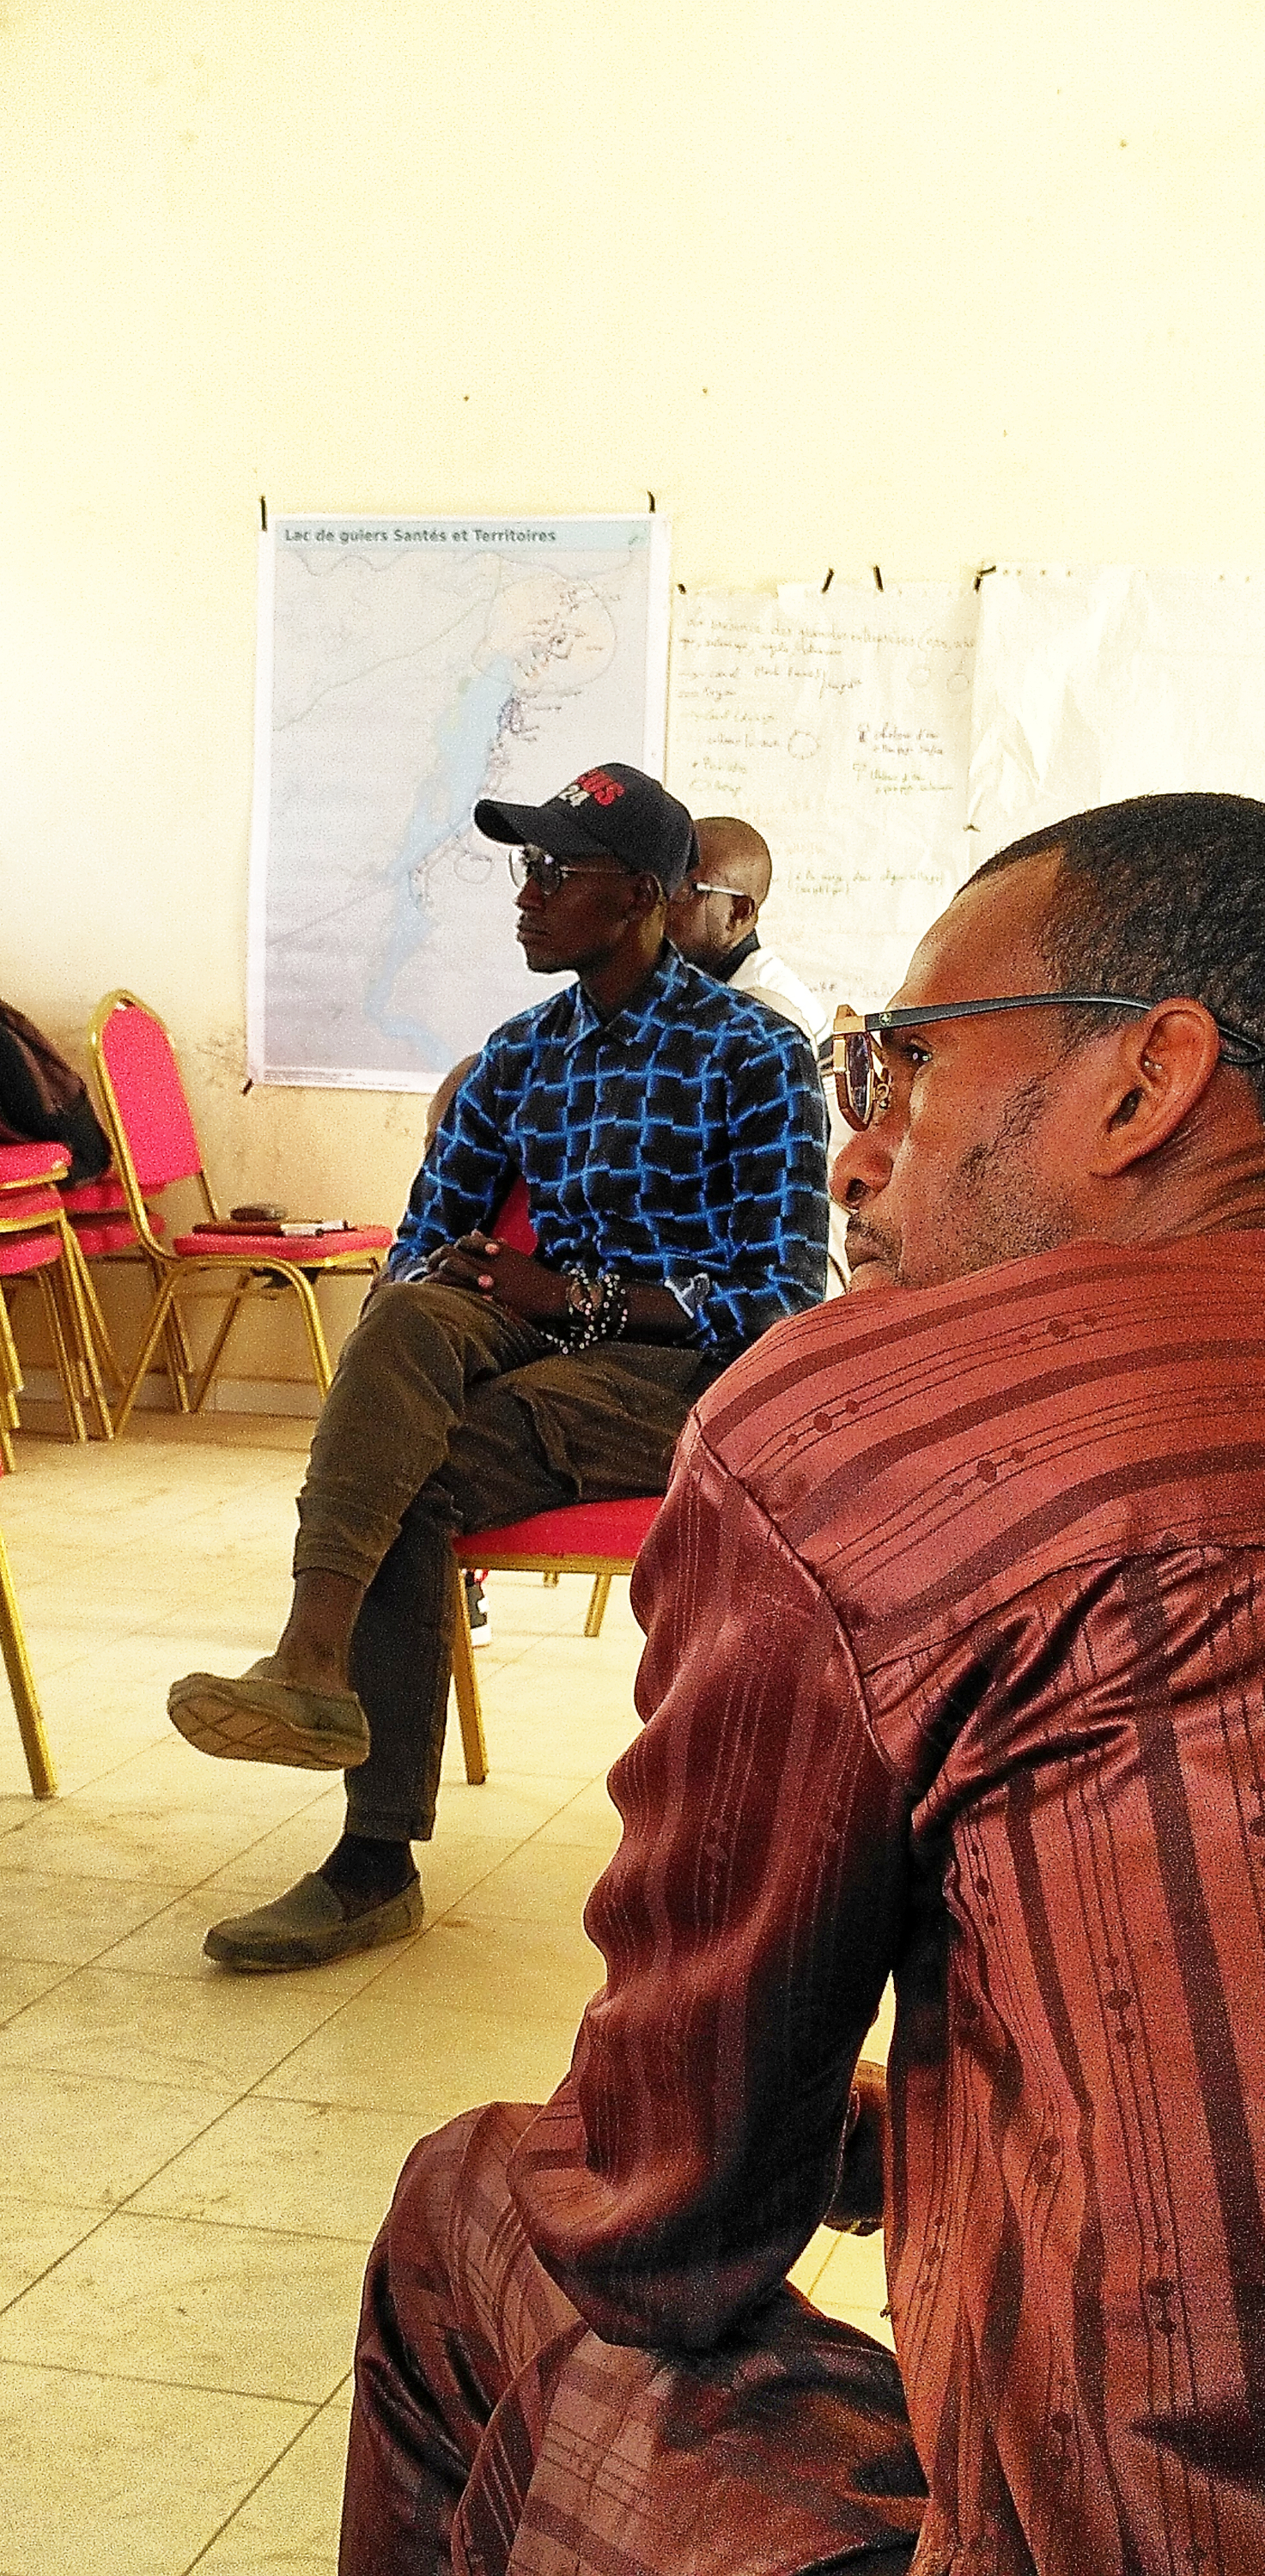
\includegraphics[height=7.5cm]{img/participants_researcher}
  \end{columns}
\end{frame}

\section{Conclusion and Outlook}

\begin{frame}[c]{Key Lessons}
  \vspace{-0.5cm}
  \begin{columns}[onlytextwidth,T]
    \column{\dimexpr\linewidth-30mm-5mm}

    \begin{itemize}
      \item \textbf{Progressive and non-linear alignments}: from dispersed elements to stabilized assemblages.  
      \item \textbf{Central role of affects and concrete dispositifs} (e.g. fodder plots, fish ponds) in triggering transformation.  
      \item \textbf{Limits}: discordant temporalities between local urgencies and long-term prospective horizons.  
    \end{itemize}

    \vspace{0.3cm}
    → Transformation emerges through situated practices, affective experiences, and negotiated alignments.

    \column{30mm}
    \vspace{1.5cm}
    % Optional illustrative icon
    % \includegraphics[height=3.5cm]{img/key_lessons.png}
  \end{columns}
\end{frame}


\begin{frame}[c]{General Conclusion}
  \vspace{-0.5cm}
  \begin{columns}[onlytextwidth,T]
    \column{\dimexpr\linewidth-30mm-5mm}

    \begin{itemize}
      \item Reducing the \textbf{“Promethean gap”} (Anders, 1957) by situating global concepts in local material and affective contexts.  
      \item \textbf{Living Labs} as genuine \textbf{laboratories of systemic transformation}.  
      \item Opening perspectives: redistribution of \textbf{capacities to act} and co-construction of \textbf{shared imaginaries}.  
    \end{itemize}

    \vspace{0.3cm}
    → From abstract slogans to situated practices that enable transformation.

    \column{30mm}
    \vspace{1.5cm}
    % Optional closing visual
    % \includegraphics[height=3.5cm]{img/conclusion.png}
  \end{columns}
\end{frame}


%-=-=-=-=-=-=-=-=-=-=-=-=-=-=-=-=-=-=-=-=-=-=-=-=
%	FRAME: MERCI DE VOTRE ATTENTION
%-=-=-=-=-=-=-=-=-=-=-=-=-=-=-=-=-=-=-=-=-=-=-=-=
{
\usebackgroundtemplate{
\includegraphics[width=\paperwidth]{img/arroseur_diohine.JPG}}%
\begin{frame}
  \vspace{-1em}
  \begin{minipage}[t][.8\textheight]{\textwidth}
    \color{\cnGrey}{\LARGE{Thank you for your attention}}

    \vfill

  %\hfill \small{Photo credit : Thomas m-louis. sur \includegraphics[height=0.55cm]{img/flickr_logo}}
  \end{minipage}
  \vspace{-3.5em}
  \centering
	You can find this presentation on github\includegraphics[height=0.85cm]{img/github}

\end{frame}
}


\end{document}